\section{Threat catalogs: the OWASP MCP Top 10 and MITRE ATLAS}
\label{sec:threats}

The flaw in the MCP Inspector (\cref{sec:inspector}) let a web page run commands on a developer's
machine because one component did not check its caller. This section first defines the terms that
separate such a defect from an adversary's use of it. It then introduces two public catalogs: the
OWASP MCP Top 10, which lists the risks of MCP deployments so that an engineer can audit a
deployment part by part, and MITRE ATLAS, which records the techniques that adversaries use against
AI systems. The next two sections (\cref{sec:attacks,sec:mitigations}) are organized by ATLAS's
techniques and mitigations, so its terms are needed to read them.

\subsection{From a design smell to a threat}
\label{sec:threats-terms}

The terms smell, fault, weakness and vulnerability describe a defect in a design, and the term
threat describes what an adversary does with such a defect. We define each term and illustrate it
with the Inspector flaw of \cref{sec:inspector}. In that flaw, the proxy, the Inspector's local
process that starts MCP servers for its web client, accepted requests from any caller.
\bi
\item \textbf{Smell.} A smell is a symptom of weak design: a property that makes a defect likely
without being a defect itself. In the Inspector, a local proxy accepted a connection from any
caller. Accepting a connection does no harm by itself, but it lets any caller reach the functions
behind it.
\item \textbf{Fault.} A fault is a defect that produces wrong behavior at run time. The proxy
launched a server process, that is, ran a command, for a request that carried no authentication.
This behavior is the defect, because a request from an unknown caller starts a program on the
developer's machine.
\item \textbf{Weakness.} A weakness is a class of fault: a kind of mistake that many products can
make. CWE, the catalog of weakness classes, lists this one as CWE-306, Missing Authentication for
Critical Function \citep{cwe-306}.
\item \textbf{Vulnerability.} A vulnerability is a reported instance of a weakness in a particular
product. A CVE identifier names one reported vulnerability, and this one is CVE-2025-49596 in the
MCP Inspector. Its advisory rates its severity at 9.4 on the 0 to 10 CVSS 4.0 scale
\citep{ghsa-7f8r-inspector}.
\item \textbf{Threat.} A threat is the action an adversary takes with a vulnerability. In the
Inspector flaw, a web page that the developer visited could launch commands on the developer's
machine, as Oligo Security demonstrated \citep{lumelsky2025inspector}. MITRE ATLAS, a catalog of the
methods that adversaries use against AI systems (\cref{sec:threats-atlas}), describes actions of
this kind.
\ei

\Cref{tab:threats-terms} sets the terms side by side, with the catalog that records each one. Its
last column, read from top to bottom, follows the Inspector flaw from a proxy that trusted any
caller to a web page that could launch commands on the developer's machine.

\begin{table*}[tb]
  \caption{The terms for a flaw and its use, each with the catalog that records it and its
  instance in the MCP Inspector flaw. Smell, fault, weakness and vulnerability describe the
  defect, and threat describes the adversary's action.}
  \label{tab:threats-terms}
  \begin{adjustbox}{width=\textwidth}\begin{tabularx}{\textwidth}{L{0.13\textwidth}L{0.27\textwidth}L{0.08\textwidth}X}
    \toprule
    \textbf{Term} & \textbf{Meaning} & \textbf{Catalog} & \textbf{In the Inspector flaw} \\
    \midrule
    \textbf{Smell} & A symptom of weak design & None & A local proxy accepted a connection from any caller. \\
    \textbf{Fault} & A defect that produces wrong behavior at run time & None & The proxy launched a server process for an unauthenticated request. \\
    \textbf{Weakness} & A class of fault & CWE & CWE-306, missing authentication for a critical function. \\
    \textbf{Vulnerability} & A reported instance in a product & CVE & CVE-2025-49596 in the MCP Inspector. \\
    \textbf{Threat} & The action an adversary takes with it & ATLAS & A web page the developer visited could launch commands on the developer's machine. \\
    \bottomrule
  \end{tabularx}\end{adjustbox}
\end{table*}

Each term calls for a different response. A smell is removed by changing the design. A fault is
removed by correcting the code that misbehaves. A weakness class tells reviewers what to look for
in any product. A vulnerability is fixed by releasing a corrected version, as version 0.14.1 of the
Inspector did. A threat is countered by mitigations that stop or expose the adversary's action
(\cref{sec:mitigations}). We use the word threat only in this sense, for an adversary's action.

The same terms apply to our own harness. The guarantees table of Lecture~4
(\cref{tab:recap-guarantees}) records, for each guarantee of \msa{}, the component that enforces
it, and it leaves reads unenforced. A defender reads that table to find what is not yet enforced,
and an attacker reads the same rows as openings. Each unenforced row marks a fault in our harness.
For example, \demoref{search} can read files outside the workspace at run time, because it skips
the path check. If such a fault were found in a released product and reported, it would be a
vulnerability, and an adversary who used it would carry out a threat.

\subsection{The OWASP MCP Top 10}
\label{sec:threats-owasp}

The \textbf{OWASP MCP Top 10} is a list of ten risks of MCP deployments, written so that an
engineer can audit a deployment against it. It is published by \textbf{OWASP}, the Open Worldwide
Application Security Project, a nonprofit community that publishes security guidance. The list is
at version 0.1, a beta \citep{owasp-mcp-top10}.

The list is young and still changing. Its entries were first written in November 2025 and revised
during 2026. Its sixth entry, Intent Flow Subversion, was earlier titled ``Prompt Injection via
Contextual Payloads'', and some project pages still show that title.

Each risk has its own entry, a page that describes the risk and adds a checklist and prevention
steps:
\bi
\item \textbf{A ``vulnerable if'' checklist.} The checklist gives four to twelve conditions under
which a deployment is exposed to the risk, such as components installed without any check of where
they came from.
\item \textbf{Prevention steps.} The prevention steps are measures that remove those conditions,
such as pinning each component to a known version.
\ei
An entry therefore answers a defender's question about a deployment as it is configured: is it
open to this risk? An entry does not describe an attack as a sequence of steps.

To read the list against a deployment, we group the risks by the part of the deployment that each
one acts on (\cref{fig:threats-owasp}). The grouping is the course's own: OWASP lists its ten risks
without any grouping. The parts are those of \cref{sec:mcp}. The host holds the model's context and
the MCP client, the server runs the tools, and tool definitions and tool results pass between them.
\bi
\item \textbf{Host and model context.} Tool Poisoning, Intent Flow Subversion, and Context
Injection \& Over-Sharing act on what the model reads: a tool definition, a tool result, and
context shared between users or sessions.
\item \textbf{Server side.} Software Supply Chain Attacks \& Dependency Tampering acts on the
package registry, a public store from which the server's package is installed and updated, and on
the packages it delivers. Command Injection \& Execution acts on the server's tool code. Shadow MCP
Servers are servers that the organization's security team never reviewed or recorded.
\item \textbf{Credentials and identity.} Token Mismanagement \& Secret Exposure, Privilege
Escalation via Scope Creep, and Insufficient Authentication \& Authorization act on the tokens and
keys that the host and the server use, and on their scopes. A token's scope is the set of actions
that the token permits, and scope creep is the gradual widening of that set.
\item \textbf{Logging.} Lack of Audit and Telemetry acts on the record of what happened. Without
logs, nobody can reconstruct an attack.
\ei

The server side includes the path by which a server reaches its users. One such public store is npm,
the package registry for JavaScript. A package registry is unrelated to the dispatcher's
registry of Lecture~4, which maps tool names to functions. The \textbf{software supply chain} of a
component is the set of packages, package registries and updates through which the component
reaches its users. An MCP server is often installed and updated from a package registry, so the
registry and every update it delivers belong to the server's supply chain.

\Cref{fig:threats-owasp} draws one deployment and attaches each risk to the part it acts on. The
credentials bar runs under the whole exchange, because both the host and the server hold tokens and
keys. The dashed box stands for a server that the security team never reviewed or recorded. No
risk is attached
to the user or to the MCP client. The risks sit where the model reads, where code runs and comes
from, where credentials are held, and where events are recorded.

\begin{figure*}[tb]
  \centering
  \definecolor{riskink}{HTML}{28285E}
  \begin{adjustbox}{width=\textwidth}
  \begin{tikzpicture}[
      sm/.style={font=\sffamily\scriptsize},
      card/.style={draw=ibmfg!50, rounded corners=1.5pt, fill=white, font=\sffamily\scriptsize,
                   inner sep=2pt, minimum height=5mm, minimum width=22mm, align=center},
      risk/.style={font=\sffamily\scriptsize\bfseries, text=riskink, align=center, inner sep=2pt,
                   fill=white, draw=riskink, line width=0.6pt, rounded corners=2pt},
      stem/.style={draw=riskink, line width=0.6pt},
      zone/.style={draw=ibmfg!70, dashed, rounded corners=3pt},
    ]
    % the deployment: user, host with model and MCP client, the exchange, the server, the registry
    \node[gnode, minimum width=12mm] (user) at (0.8,3.3) {user};
    \draw[zone] (1.9,2.3) rectangle (6.85,4.3);
    \node[sm, font=\sffamily\scriptsize\bfseries, anchor=north west] at (1.95,4.28) {host};
    \node[mnode, minimum width=15mm, minimum height=8mm] (model) at (2.95,3.3) {model};
    \node[mnode, minimum width=21mm, minimum height=8mm] (client) at (5.5,3.3) {MCP client};
    \draw[flow] (user.east) -- (model.west);
    \draw[flow] (model.east) -- (client.west);

    \draw[back] (10.0,3.85) -- (6.6,3.85);
    \draw[flow] (6.6,3.3) -- (10.0,3.3);
    \draw[back] (10.0,2.75) -- (6.6,2.75);
    \node[card] (defn) at (8.3,3.85) {tool definition};
    \node[card] (resl) at (8.3,2.75) {tool result};
    \node[lab] at (8.3,3.3) {\texttt{tools/call}};

    \node[rnode, anchor=south west, minimum width=28mm, minimum height=16mm, inner sep=0pt] (srv) at (10.0,2.5) {};
    \node[font=\sffamily\footnotesize\bfseries, anchor=north west, inner sep=0pt] at (10.12,4.02) {MCP server};
    \node[draw=ibmfg!60, fill=white, rounded corners=1.5pt, sm, inner sep=3pt, minimum width=20mm] (tool) at (11.4,3.0) {tool code};
    \node[rnode, minimum width=18mm] (reg) at (15.2,3.65) {package\\registry};
    \draw[flow] (reg.west) -- (12.8,3.65) node[midway, above=0.5pt, sm, inner sep=1pt] {install};

    % credentials and logs, under the whole exchange
    \draw[draw=riskink!45, fill=riskink!8, rounded corners=2pt] (1.9,0.08) rectangle (13.0,0.5);
    \node[font=\sffamily\scriptsize\bfseries, text=riskink] at (7.45,0.29) {credentials: tokens, keys and scopes};
    \node[rnode, anchor=south, minimum width=20mm, inner sep=3pt] (logs) at (15.2,0.08) {logs};

    % host and model context
    \node[risk] (p1) at (4.35,5.2) {Context Injection \& Over-Sharing};
    \draw[stem] (p1.south) -- (4.35,4.3);
    \node[risk] (p2) at (8.3,4.8) {Tool Poisoning};
    \draw[stem] (p2.south) -- (defn.north);
    \node[risk] (p3) at (8.3,1.85) {Intent Flow\\Subversion};
    \draw[stem] (p3.north) -- (resl.south);

    % server side
    \node[risk] (p4) at (11.4,5.0) {Command Injection\\\& Execution};
    \draw[stem] (p4.south) -- (11.4,4.1);
    \node[risk] (p5) at (15.2,5.05) {Software Supply\\Chain Attacks\\\& Dependency\\Tampering};
    \draw[stem] (p5.south) -- (reg.north);
    \node[risk, dashed, minimum width=25mm, minimum height=9mm] at (15.2,2.45) {Shadow\\MCP Servers};

    % credentials and identity
    \node[risk, anchor=south] at (3.9,0.5) {Token Mismanagement\\\& Secret Exposure};
    \node[risk, anchor=south] at (7.45,0.5) {Privilege Escalation\\via Scope Creep};
    \node[risk, anchor=south] at (11.0,0.5) {Insufficient Authentication\\\& Authorization};

    % logging
    \node[risk] (l1) at (15.2,1.45) {Lack of Audit\\and Telemetry};
    \draw[stem] (l1.south) -- (logs.north);
  \end{tikzpicture}
  \end{adjustbox}
  \caption{The ten risks of the OWASP MCP Top 10, each placed by the course on the part of an MCP
  deployment it acts on. The model box stands for the context that the host assembles for the
  model. The dashed box stands for a server that the security team never reviewed or recorded.}
  \label{fig:threats-owasp}
\end{figure*}

\subsection{Documented cases of the risks}
\label{sec:threats-cases}

For each risk, we name the best-supported documented public case that we found, read at its primary
source, so that the risk is tied to something that happened (\cref{tab:threats-cases}). Lack of
Audit and Telemetry is the one risk for which we found no case, as the end of this subsection
explains. The table gives each risk with its OWASP identifier, a one-sentence summary of what goes
wrong, and the case. The summaries are our own wording.

\begin{table*}[tb]
  \caption{The risks of the OWASP MCP Top 10 in OWASP's order, with our summary of each and the
  documented case we chose for it, where we found one. The summaries and the choice of cases are
  the course's.}
  \label{tab:threats-cases}
  \begin{adjustbox}{width=\textwidth}\begin{tabularx}{\textwidth}{L{0.065\textwidth}L{0.2\textwidth}L{0.33\textwidth}X}
    \toprule
    \textbf{ID} & \textbf{Risk} & \textbf{What goes wrong} & \textbf{Documented case} \\
    \midrule
    MCP01 & \textbf{Token Mismanagement \& Secret Exposure} & A token stored in configuration, logs or model memory can be read and reused. & GitHub advisory, January 2026 (research by Check Point): Claude Code project files leaked an API key. \\
    MCP02 & \textbf{Privilege Escalation via Scope Creep} & An agent's permissions widen over time until one mistaken call can do serious damage. & GitHub advisories, December 2025: the Git MCP server ignored its repository boundary. \\
    MCP03 & \textbf{Tool Poisoning} & A tool's description hides an instruction, so the model obeys the tool's author. & Invariant Labs, April 2025: hidden instructions in a tool description. \\
    MCP04 & \textbf{Software Supply Chain Attacks \& Dependency Tampering} & A server package the user installed, or later updated, carries the attacker's code. & Koi Security, September 2025: postmark-mcp copied every email to the attacker. \\
    MCP05 & \textbf{Command Injection \& Execution} & A tool passes model-written text to a shell or database without checking it. & JFrog, July 2025: mcp-remote ran attacker commands. \\
    MCP06 & \textbf{Intent Flow Subversion} & Instructions hidden in a file or tool result redirect the agent's plan. & Invariant Labs, May 2025: a GitHub issue made an agent leak private repositories. \\
    MCP07 & \textbf{Insufficient Authentication \& Authorization} & A server or client accepts any caller without checking identity or permission. & Oligo Security, June 2025: the Inspector proxy accepted unauthenticated requests. \\
    MCP08 & \textbf{Lack of Audit and Telemetry} & Tool calls and context changes go unrecorded, so nobody can reconstruct an attack. & No MCP-specific incident found. \\
    MCP09 & \textbf{Shadow MCP Servers} & A team runs an MCP server that the organization's security staff never reviewed or recorded. & Knostic, July 2025: a scan found 1,862 MCP servers open to the internet. \\
    MCP10 & \textbf{Context Injection \& Over-Sharing} & Context shared between users or sessions leaks data or carries injected instructions forward. & BleepingComputer, June 2025: Asana's MCP server exposed one organization's data to another. \\
    \bottomrule
  \end{tabularx}\end{adjustbox}
\end{table*}

The cases differ in the kind of evidence they provide, and the kind decides what a case shows.
\bi
\item \textbf{In the wild.} A case in the wild is an attack observed against real users, here a
malicious package that users installed. The package postmark-mcp, which copied every email sent
through it to its author, is the one case of this kind \citep{dardikman2025postmark}, and
\cref{sec:threats-postmark} reads it in detail. Such a case shows that adversaries carry out the
attack against real users.
\item \textbf{Vendor advisory.} A vendor advisory is a vendor's published notice of a flaw that it
has fixed. Claude Code, Anthropic's coding agent, reads configuration files stored in a project,
and a malicious project could make it leak the user's API key (CVE-2026-21852, January 2026)
\citep{ghsa-jh7p-claude-code}. The same research by Check Point found an earlier flaw,
CVE-2025-59536, in which a project's files ran commands before Claude Code asked the user whether
to trust the project \citep{lyons2026claudecode}. The Git MCP server ignored the repository it was
configured to stay inside (advisories of December 2025)
\citep{ghsa-j22h-mcp-server-git,lakshmanan2026gitmcp}. The package mcp-remote, which lets hosts
connect to remote MCP servers, ran operating-system commands chosen by an attacker when it
connected to an untrusted server (CVE-2025-6514, July 2025) \citep{peles2025mcpremote}. In this
case, the commands came from a malicious server rather than from the model. The Inspector flaw of
\cref{sec:inspector} is a case of the same kind. An advisory shows that a flaw existed in the named
versions and was fixed. It does not show that anyone exploited it.
\item \textbf{Proof of concept.} A proof of concept is a demonstration, by researchers, that an
attack can be carried out. Invariant Labs hid instructions in a tool description and showed that
the model followed them \citep{beurerkellner2025toolpoisoning}. It also showed that a GitHub issue
written by an attacker could make an agent leak the contents of private repositories
\citep{milanta2025githubmcp}. Such a case shows that the attack works under the researchers'
conditions.
\item \textbf{Vendor scan.} A vendor scan is a measurement, by a security company, of many
deployments at once. Knostic found 1,862 MCP servers open to the internet. It checked a sample of
119 by hand, and every one of them listed its tools to a caller that gave no credentials
\citep{goldberg2025mcpservers}. A scan measures exposure. It cannot tell whether the organization
that runs a server had reviewed and recorded it, and only a server that was never reviewed or
recorded is a shadow server.
\item \textbf{Vendor bug.} A vendor bug is a flaw that the vendor itself found and disclosed, with
no attack reported. Asana found in June 2025 that its MCP server had exposed one organization's
data to another \citep{toulas2025asana}. Such a case shows that the risk occurred, through the
vendor's own mistake.
\ei

Lack of Audit and Telemetry has no case. For this risk, a short search on October 8, 2026 found
guidance and survey statistics. It found no MCP-specific incident. An incident may exist that the
search missed.

\subsection{One incident read through both catalogs}
\label{sec:threats-postmark}

The two catalogs answer different questions about the same incident. OWASP asks which conditions
made a deployment vulnerable, and ATLAS records what the adversary did, step by step. We read the
postmark-mcp incident of September 2025 through each.

Postmark is a service that sends email for organizations through an API, and its MCP server lets AI
agents send email through it. An adversary impersonated Postmark on npm by publishing a package
named postmark-mcp, a name that Postmark had not registered there. The first versions behaved like
a legitimate server. Version 1.0.16 added one line of code, which made the adversary's address a
blind-copy (BCC) recipient of every email sent through the package's tool
\citep{dardikman2025postmark,lakshmanan2025postmark}. A BCC recipient receives a copy of a message,
and the other recipients do not see the address.

In \cref{fig:threats-postmark}, a strip across the top summarizes the incident. Below it, the left
half lists the conditions of the deployment that OWASP's entry names, and the right half lists the
adversary's steps in order, as ATLAS records them.

\begin{figure*}[tb]
  \centering
  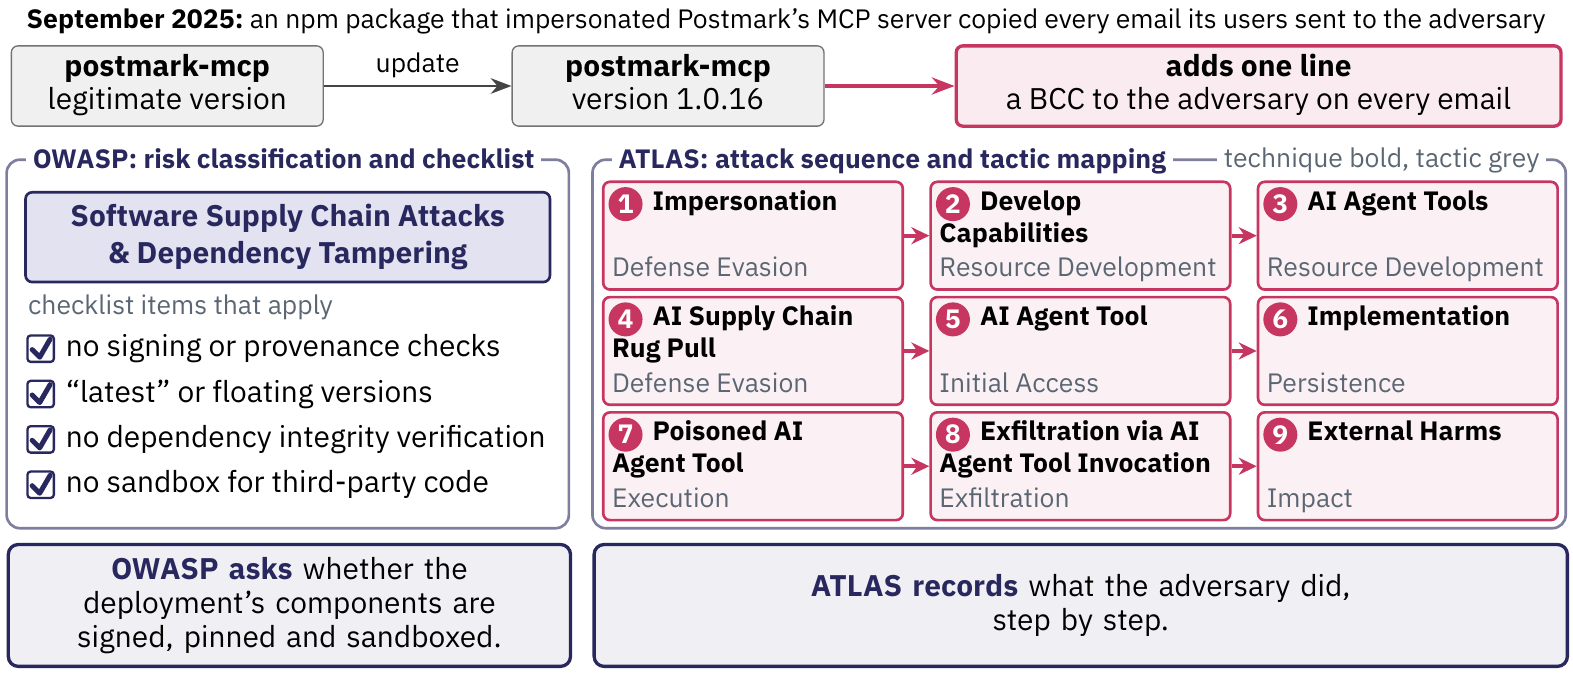
\includegraphics[width=\textwidth]{figures/deck/ca32441fe6.png}
  \caption{The postmark-mcp incident read through both catalogs: on the left, the OWASP entry that
  fits and the checklist items that applied, and on the right, the nine steps of the ATLAS case
  study, each a technique (bold) above its tactic (grey). Where a step is a sub-technique, its box
  shows only the sub-technique's name, and the text gives the full names. The mapping to the OWASP
  entry and the ticked items are the course's proposal.}
  \label{fig:threats-postmark}
\end{figure*}

\paragraph{The OWASP view.} OWASP's entry Software Supply Chain Attacks \& Dependency Tampering
fits the incident. Its first example scenario, ``Trojanized Plugin'', reads: ``A popular
open-source connector gains a malicious update. It silently exfiltrates customer support transcripts
to an adversary-controlled endpoint'' \citep{owasp-mcp-top10}. We propose that the following items
of the entry's checklist applied to the incident:
\bi
\item \textbf{No provenance check.} ``The system installs MCP connectors or plugins without signing
/ provenance checks.'' Without such a check, nothing verifies that a package comes from the
vendor it names.
\item \textbf{Floating versions.} ``Teams use `latest' or floating version references.'' A
deployment that follows the latest version receives an update such as 1.0.16 without anyone
choosing it.
\item \textbf{No integrity check.} ``There is no dependency integrity verification (hash,
signature, attestation).'' Without it, nothing compares the installed code with a copy known to be
good.
\item \textbf{No sandbox.} ``No sandboxing isolates third-party components.'' Without a sandbox, a
package's code runs with whatever access its process has.
\ei
OWASP does not mention postmark-mcp, and its own summary of the Tool Poisoning entry lists rug
pulls, a legitimate release followed by a malicious update, so the incident could also be filed
there. Under either entry, the OWASP view gives an engineer a question to ask of a deployment: are
its components signed, pinned to a version and sandboxed?

\paragraph{The ATLAS view.} ATLAS records the same incident as a case study, a documented attack
mapped to the techniques it used \citep{atlas-cs0053-postmark}. Each step names the method the
adversary used, which ATLAS calls a technique, and the goal the step served, which ATLAS calls a
tactic (\cref{sec:threats-atlas} defines both terms). A name of the form ``technique:
sub-technique'' names a narrower variant of a technique, which ATLAS calls a sub-technique. The
case study lists nine ordered steps:
\be
\item \textbf{Impersonation} (Defense Evasion). The adversary published a legitimate version under
the name postmark-mcp, so users took the package for Postmark's own.
\item \textbf{Develop Capabilities} (Resource Development). The adversary modified the server to add
the adversary's address to the BCC line of every email.
\item \textbf{Publish Poisoned AI Artifacts: AI Agent Tools} (Resource Development). The adversary
published the malicious version to npm.
\item \textbf{AI Supply Chain Rug Pull} (Defense Evasion). Because users adopted a legitimate
version first, the malicious one avoided the scrutiny that new tools receive.
\item \textbf{AI Supply Chain Compromise: AI Agent Tool} (Initial Access). Organizations that
upgraded to version 1.0.16 received the malicious version through the package registry.
\item \textbf{AI Agent Tool Poisoning: Implementation} (Persistence). The malicious line sat in the
tool's code, its implementation, which the model never reads (\cref{sec:attacks}). Once configured
with an organization's agents, the poisoned server stayed in place.
\item \textbf{User Execution: Poisoned AI Agent Tool} (Execution). When users asked their agents to
use the server's tools, the malicious code ran.
\item \textbf{Exfiltration via AI Agent Tool Invocation} (Exfiltration). Every email sent through
the tool was copied to the adversary.
\item \textbf{External Harms} (Impact). The copied emails could reveal private information about the
organization's clients, and the list of its clients.
\ee
A tactic can serve more than one step: Defense Evasion serves the first and the fourth steps, and
Resource Development the second and the third.

The case study limits the loss to users who upgraded to the malicious version and kept using the
tool.

\paragraph{The two views compared.} Each catalog supplies what the other lacks.
\bi
\item \textbf{OWASP} gives a checklist of vulnerable conditions and steps that prevent them, which an
engineer can apply to a deployment before any attack. It orders no steps of an attack, and it rates
no evidence: an entry does not say whether its scenarios have been seen in real attacks.
\item \textbf{ATLAS} records what an adversary did, in order, with the goal of each step, and it
types each case study as a real attack or a demonstration. It gives no checklist of vulnerable
conditions, and it maps no mitigation to several steps of this incident, among them AI Supply
Chain Rug Pull and AI Agent Tool Poisoning (\cref{sec:mitigations}).
\ei

\subsection{MITRE ATLAS and its terms}
\label{sec:threats-atlas}

MITRE ATLAS describes each step of an attack on an AI system by its goal and its method.
\textbf{MITRE ATLAS} (Adversarial Threat Landscape for AI Systems) is MITRE's knowledge base of
adversary tactics and techniques against AI-enabled systems \citep{mitre-atlas-2026}. MITRE is a
US nonprofit research organization. ATLAS is modeled on \textbf{MITRE ATT\&CK}, MITRE's knowledge
base of the same kind for ordinary computer systems. ATLAS is built from tactics, techniques,
sub-techniques, mitigations and case studies:
\bi
\item \textbf{Tactic.} A tactic is the adversary's goal at one stage of an attack, such as getting
into the system, avoiding detection or stealing data.
\item \textbf{Technique.} A technique is a method for reaching a tactic's goal. Exfiltration via AI
Agent Tool Invocation, for example, reaches the goal of stealing data by having the agent call a
tool that sends the data out.
\item \textbf{Sub-technique.} A sub-technique refines a technique to a narrower method. AI Agent
Tools refines Publish Poisoned AI Artifacts to the case in which the published artifact is a tool
for an agent, and ATLAS writes the pair as ``Publish Poisoned AI Artifacts: AI Agent Tools''.
\item \textbf{Mitigation.} A mitigation is a countermeasure mapped to the techniques it counters.
\Cref{sec:mitigations} studies the mitigations mapped to the techniques of this lecture.
\item \textbf{Case study.} A case study, such as the postmark-mcp one of
\cref{sec:threats-postmark}, is a documented attack mapped, step by step, to the techniques it
used. ATLAS types each one as an \textbf{incident}, a real attack, or an \textbf{exercise}, a
demonstration by researchers or by testers whom the system's owner authorized to attack it. The
postmark-mcp case study is an incident.
\ei

ATLAS is updated in numbered releases, and we use release 2026.09, of September 2026. Release
2026.09 holds 120 techniques and 88 sub-techniques, which together we call its 208 entries. The
same release holds 16 tactics, 40 mitigations and 73 case studies, of which 23 are incidents and 50
are exercises.

The postmark-mcp case study uses the following tactics:
\bi
\item \textbf{Resource Development.} The adversary builds resources for the attack, such as a
modified package.
\item \textbf{Defense Evasion.} The adversary avoids detection.
\item \textbf{Initial Access.} The adversary gets into the target system.
\item \textbf{Persistence.} The adversary keeps its access to the system over time.
\item \textbf{Execution.} The adversary's code runs.
\item \textbf{Exfiltration.} The adversary moves data out of the victim's systems.
\item \textbf{Impact.} The adversary manipulates, interrupts or destroys the victim's systems and
data.
\ei

ATLAS thus describes an attack by the goal and the method of each step. It connects methods to the
countermeasures that address them, where ATLAS records any, and to the incidents and exercises that
used them. A defender can therefore move from an observed step to known attacks and, where they
exist, to known defenses.

\subsection{The ATLAS matrix}
\label{sec:threats-matrix}

The ATLAS matrix arranges the techniques by the goals they serve (\cref{fig:threats-matrix}). The
\textbf{ATLAS matrix} is a table whose columns are the tactics, ordered as the stages of an attack,
and whose cells are the techniques that serve each tactic. In release 2026.09, the matrix has
sixteen columns, from Reconnaissance on the left to Impact on the right, and
\cref{fig:threats-matrix} prints them all. Each cell is a technique, and sub-techniques are not
drawn.

A technique that serves several tactics appears under each of them. For this reason, the 120
techniques of release 2026.09 fill 131 cells. AI Agent Tool Invocation, a technique that recurs
throughout this lecture, sits under three tactics.

\begin{definition}[AI Agent Tool Invocation]
\label{def:threats-invocation}
``Adversaries may use their access to an AI agent to invoke tools the agent has access to.''
\citep{mitre-atlas-2026}
\end{definition}

\textbf{AI Agent Tool Invocation} is the use of access to an agent to invoke the tools it can reach.
It appears under three tactics:
\bi
\item \textbf{Execution.} Invoking a tool runs an action, such as a command or an API call.
\item \textbf{Privilege Escalation.} An agent may hold tools and permissions that the adversary does
not, so acting through the agent gains rights the adversary lacks.
\item \textbf{Lateral Movement.} The tools connect the agent to other applications and systems, and
the adversary reaches those systems through them.
\ei
In our running example, an instruction planted in text that \msa{} reads could lead the model to
call \demoref{edit}. This is indirect prompt injection, introduced in Lecture~4: text from a source
outside the application's control reaches the model's context as an observation and steers the next
action. The adversary would then change code through the agent without holding any right to edit
that code. The call serves Execution,
because it runs an action, and Privilege Escalation, because it uses a right that the agent holds
and the adversary lacks.

\begin{figure*}[tb]
  \centering
  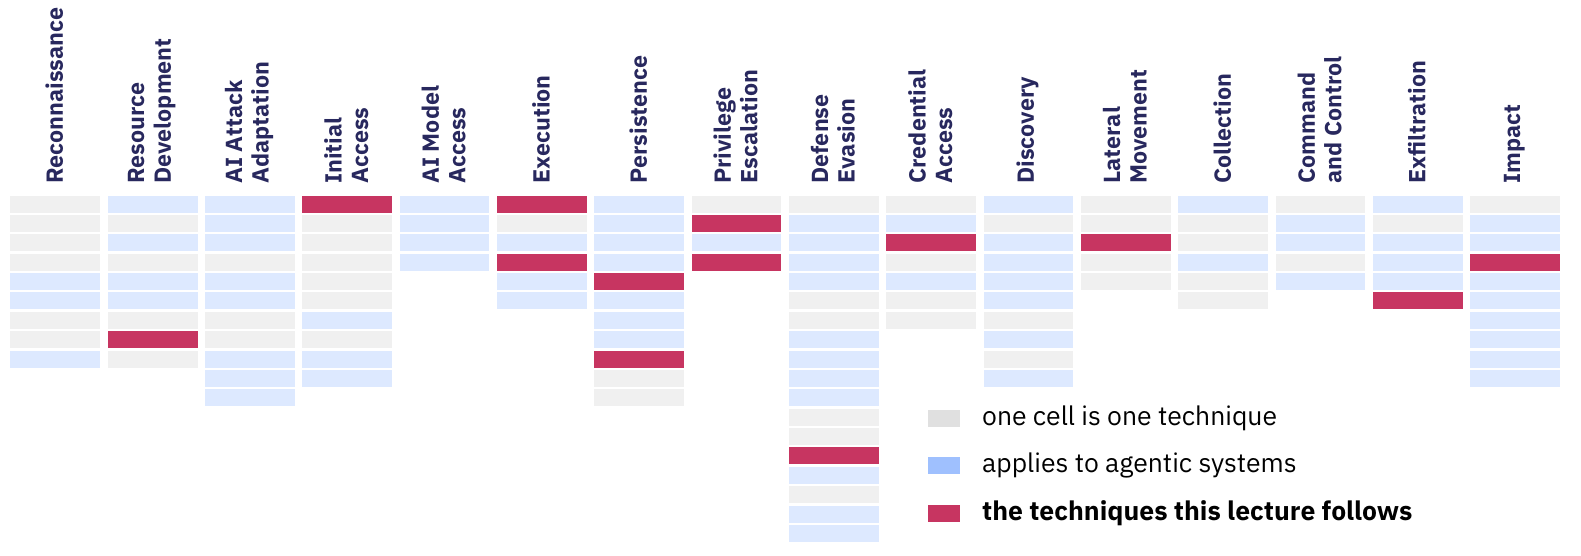
\includegraphics[width=\textwidth]{figures/deck/233b9a12ab.png}
  \caption{The ATLAS matrix of release 2026.09. Each column is a tactic, in the order of the stages
  of an attack, and each cell is a technique. Blue cells carry the Agentic AI tag, which the legend
  reads as applying to agentic systems, and magenta cells are the techniques this lecture follows.}
  \label{fig:threats-matrix}
\end{figure*}

The colors of the matrix mark two sets of techniques. Blue cells mark techniques that carry the
Agentic AI tag, which means that the platforms field of their ATLAS entry lists Agentic AI
(\cref{sec:threats-agentic} describes the field). In release 2026.09, 76 techniques carry the tag, and
they fill 82 cells. A cell whose technique this lecture follows is drawn in magenta even when the
technique carries the tag, so the figure shows 70 blue cells. The matrix draws no sub-techniques.
In the same release, another 63 sub-techniques carry the tag, and with them the tag covers the 139
entries that \cref{sec:threats-agentic} counts.

Magenta cells mark the techniques that \cref{sec:attacks,sec:mitigations} follow, listed in
\cref{tab:threats-eleven} in the order in which an attack uses them. Where the lecture follows a
sub-technique, the matrix marks its parent's cell. The lecture follows Agentic Resource
Consumption, for example, and the matrix marks the cell of its parent, Cost Harvesting. Escape to
Host is the only technique of the set without the Agentic AI tag, because ATLAS lists it only for
the Enterprise platform, which covers ordinary computer systems (\cref{sec:threats-agentic}).

\begin{table}[htbp]
  \caption{The techniques this lecture follows, in the order an attack uses them, with the tactics
  under which the ATLAS matrix places them.}
  \label{tab:threats-eleven}
  \begin{adjustbox}{width=\linewidth}\begin{tabularx}{\linewidth}{XL{0.36\linewidth}}
    \toprule
    \textbf{Technique} & \textbf{Tactic} \\
    \midrule
    \textbf{AI Agent Tool Poisoning} & Persistence \\
    \textbf{Publish Poisoned AI Artifacts: AI Agent Tools} & Resource Development \\
    \textbf{AI Supply Chain Rug Pull} & Defense Evasion \\
    \textbf{AI Supply Chain Compromise: AI Agent Tool} & Initial Access \\
    \textbf{User Execution: Poisoned AI Agent Tool} & Execution \\
    \textbf{AI Agent Tool Invocation} & Execution, Privilege Escalation, Lateral Movement \\
    \textbf{Credentials from AI Agent Configuration} & Credential Access \\
    \textbf{Exfiltration via AI Agent Tool Invocation} & Exfiltration \\
    \textbf{Escape to Host} & Privilege Escalation \\
    \textbf{AI Agent Context Poisoning} & Persistence \\
    \textbf{Cost Harvesting: Agentic Resource Consumption} & Impact \\
    \bottomrule
  \end{tabularx}\end{adjustbox}
\end{table}

\subsection{Agentic AI coverage in ATLAS}
\label{sec:threats-agentic}

The Agentic AI tag marks the ATLAS entries in which an adversary may operate on an agent, and most
tagged entries are general techniques that list other AI platforms as well. Every ATLAS entry has a
platforms field, which ATLAS describes as denoting ``the platform(s) the adversary is operating in''
\citep{mitre-atlas-2026}. Its values are Predictive AI (models that classify or predict),
Generative AI (models that generate text, images or code), Agentic AI (systems in which a model
calls tools) and Enterprise (ordinary computer systems). We say that an entry carries the
\textbf{Agentic AI tag} when its platforms field lists Agentic AI. Reading the tag as ``this
technique applies to agents'' is our interpretation of the field.

In release 2026.09, 139 of the 208 entries carry the tag, about two thirds of the catalog.
\Cref{fig:threats-agentic} counts the entries by the year in which each was created, and splits
each year's entries three ways: no tag, the tag with another AI platform, and the tag with no other
AI platform.

\begin{figure*}[tb]
  \centering
  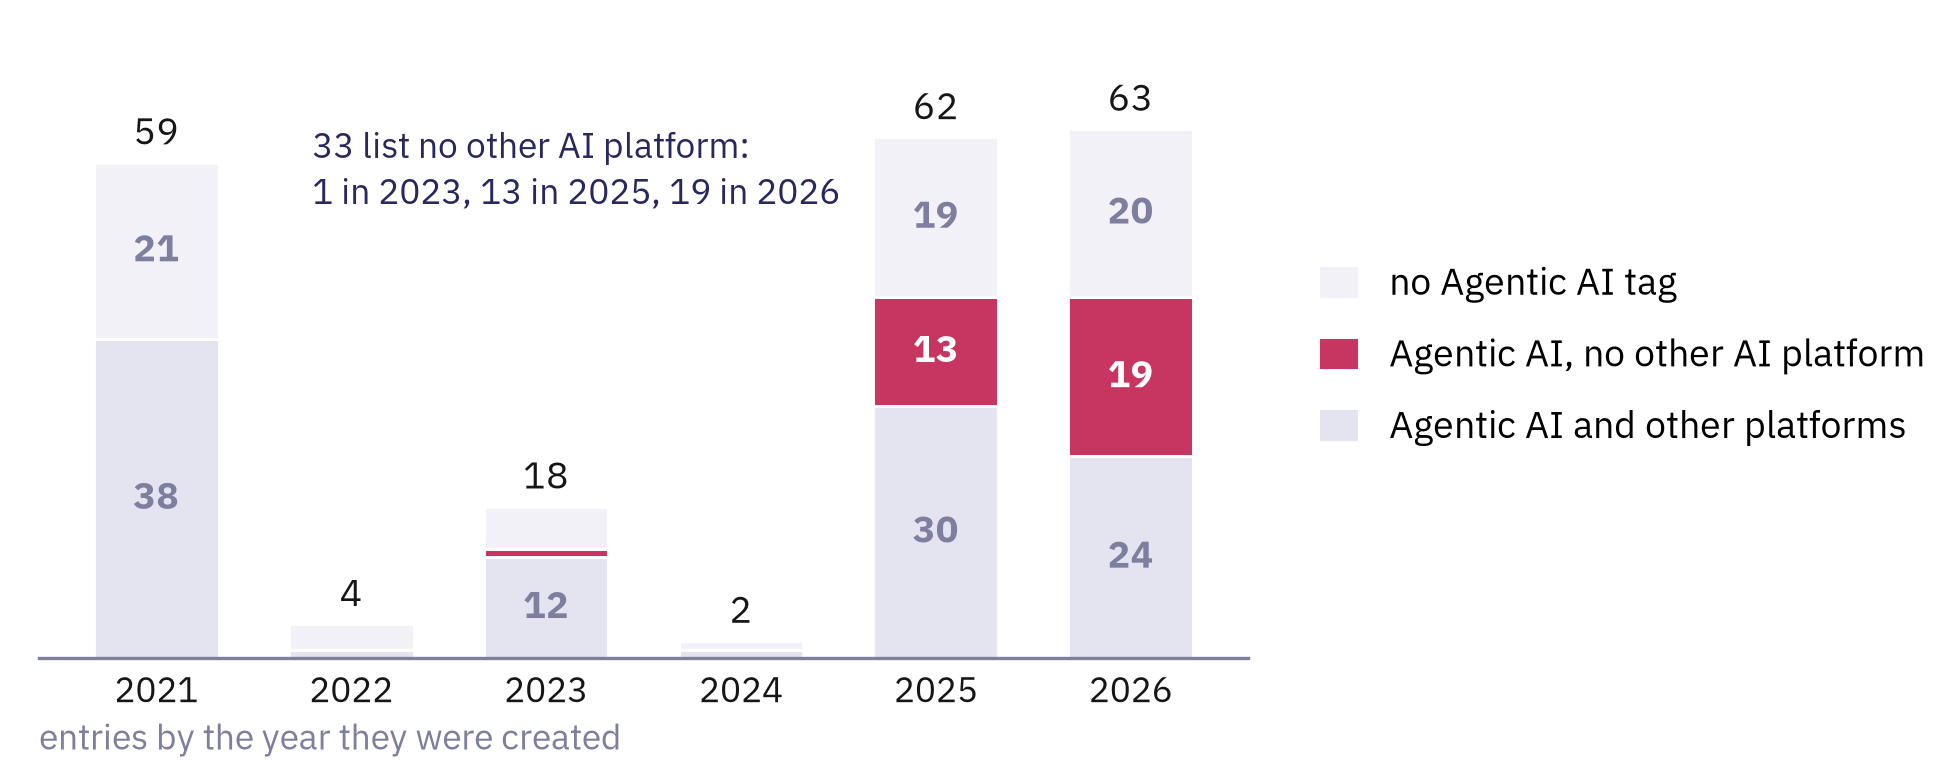
\includegraphics[width=0.85\textwidth]{figures/deck/7abcf7c40c.png}
  \caption{ATLAS entries (techniques and sub-techniques) of release 2026.09, counted by the year in
  which each was created. Each bar is split by whether the entry carries the Agentic AI tag and
  whether Agentic AI is its only AI platform. In the legend, ``other platforms'' means other AI
  platforms, so an entry that lists only Agentic AI and Enterprise counts as having no other AI
  platform.}
  \label{fig:threats-agentic}
\end{figure*}

The chart supports the following readings:
\bi
\item \textbf{Old entries carry the tag.} In release 2026.09, the 38 tagged entries created in
2021 are general-purpose techniques, and each lists Predictive AI and Generative AI as well as Agentic AI. The platforms
field did not exist when they were written. Release 2026.05 added it to every technique: ``All
techniques are updated to include one or more platforms (Predictive AI, Generative AI, Agentic AI,
Enterprise).''
\item \textbf{Few entries list no other AI platform.} In release 2026.09, only 33 entries list
no other AI platform: 29 list Agentic AI alone, and 4 list Agentic AI with Enterprise. In the same
release, the other 106 tagged entries also list Predictive AI or Generative AI, and 69 entries carry
no tag.
\item \textbf{Entries with no other AI platform are recent.} All 33 entries of release 2026.09 that
list no other AI platform were created in 2023 or later: one in 2023, 13 in 2025 and 19 in 2026.
The one from 2023 is AI Agent Tool Invocation, created in October 2023 and renamed in September
2025. Across release 2026.09, 125 of the 208 entries were created in 2025 or 2026.
\ei

On our reading, the tag therefore marks the techniques that apply to agents, and most of them were
written for AI systems in general. The entries that list no other AI platform were all created in
2023 or later, and every one except AI Agent Tool Invocation was created in 2025 or 2026. The chart
counts catalog entries. It does not count attacks. The year of an entry records when ATLAS added
the technique, which need not be when adversaries began to use it.

\subsection*{Key points}
\bi
\item A smell is a symptom of weak design, a fault is a defect that misbehaves at run time, a
weakness is a class of faults (cataloged in CWE), a vulnerability is a reported instance in a product
(identified by a CVE), and a threat is the action an adversary takes with it (described in ATLAS).
\item The OWASP MCP Top 10 (version 0.1, beta) lists ten risks of MCP deployments, each with a
``vulnerable if'' checklist and prevention steps, and the course groups them by the part of a
deployment they act on: host and model context, server side, credentials and identity, and logging.
\item A documented case shows only what its kind of evidence can show: an attack in the wild shows
that adversaries use the attack against real users, an advisory shows a fixed flaw but not its
exploitation, a proof of concept shows that an attack works under the researchers' conditions, and a
scan measures exposure.
\item OWASP gives a checklist of the conditions that make a deployment vulnerable but orders no
attack steps and rates no evidence, while ATLAS records an attack's steps in order, each a
technique under a tactic, but gives no checklist.
\item In ATLAS, a tactic is the adversary's goal at one stage, a technique is a method for reaching
it, a sub-technique refines a technique, a mitigation counters techniques, and a case study maps a
documented incident or exercise to the techniques it used.
\item The ATLAS matrix places each technique under every tactic it serves, so AI Agent Tool
Invocation, the use of an agent's access to invoke its tools, appears under Execution, Privilege
Escalation and Lateral Movement.
\item Most ATLAS entries that carry the Agentic AI tag are general AI techniques that also list
other AI platforms, and those that list no other AI platform were all created in 2023 or later (in
release 2026.09, 139 of 208 entries carry the tag, and 33 list no other AI platform).
\ei
